\section{第三章 Markov过程}
\begin{problem}{3.1}
对Markov链$X_n,n\geqslant 0$,试证条件\[\p(X_{n+1}=j|X_0=i_0,\dots ,X_{n-1}=i_{n-1},X_n=i)=\p(X_{n+1}=j|X_n=i)\]
等价于对所有时刻$n,m$及所有状态$i_0,\dots , i_n,j_1,\dots ,j_m$有
\[\begin{aligned}
		  & \p(X_{n+1}=j_1,\dots ,X_{n+m}=j_m|X_0=i_0, \dots , X_n=i_n) \\
		= & \p(X_{n+1}=j_1,\dots ,X_{n+m}=j_m|X_n=i_n)
	\end{aligned}\]
\end{problem}
\begin{solution}
	$\Leftarrow $只需令$m=1$\\
	$\Rightarrow $由$\mathbf{P}_{27}(3.4)$可知
	\[\begin{split}
			& \quad P\{X_{n+1} = j_1, \cdots, X_{n+m} = j_m | X_0 = i_0, \cdots, X_n = i_n\}\\
			& = P\{X_{n+1} = j_1, \cdots, X_{n+m} = j_m , X_0 = i_0, \cdots, X_n = i_n\} / P\{X_0 = i_0, \cdots, X_n = i_n\}\\
			& = P\{X_0 = i_0\} \cdot P_{j_1j_2} \cdots P_{j_{m-1}j_m} P_{i_0i_1} \cdots P_{i_1j_1} / [P\{X_0 = i_0\} \cdot P_{i_0i_1} \cdots P_{i_{n-1}i_n}\\
			& = P\{X_n = i\} \cdot P_{j_1j_2} \cdots P_{j_{m-1}j_m} P_{i_nj_1} / P\{X_n = i_n\}\\
			& = P\{X_{n+1} = j_1, \cdots, X_{n+m} = j_m | X_n = i_n\}\\
		\end{split}\]
\end{solution}

\begin{problem}{3.2}
考虑状态 $ 0,1,2 $ 上的一个Markov链$X_n, n \geqslant 0$, 它有转移概率矩阵
\[\bm{P} = \begin{pmatrix}
		0.1 & 0.2 & 0.7 \\
		0.9 & 0.1 & 0   \\
		0.1 & 0.8 & 0.1
	\end{pmatrix}\]
初始分布为$p_0 = 0.3, p_1 = 0.4, p_2 = 0.3$, 试求概率$P\{X_0 = 0, X_1 = 1, X_2 = 2\}$.
\end{problem}
\begin{solution}
	\[\p\{X_0 = 0, X_1 = 1, X_2 = 2\} = p_0P_{01}P_{12} = 0.3 \times 0.1 \times 0 = 0\]
\end{solution}

\begin{problem}{3.3}
信号传送问题. 信号只有 $0,1$ 两种, 分为多个阶段传输. 在每一步上出错的概率为$\alpha$. $X_0 = 0$是送出的信号, 而$X_n$是在第$n$步接收到的信号. 假定$X_n$为一Markov链,它有转移概率矩阵$P_{00} = P_{11} = 1-\alpha,\,P_{01} = P_{10} = \alpha,\, 0<\alpha <1$.试求
\begin{enumerate}[label=(\alph*)]
	\item 两步均不出错的概率$\p\{X_0 = 0, X_1 = 0, X_2 = 0\}$;
	\item 两步传送后收到正确信号的概率;
	\item 五步之后传送无误的概率$\p\{X_5 = 0 | X_0 = 0\}$.
\end{enumerate}
\end{problem}
\begin{solution}
	\begin{enumerate}[label=(\alph*)]
		\item $\p\{X_0 = 0, X_1 = 0, X_2 = 0\} = p_0P_{00}P_{00} = 1 \cdot (1-\alpha) \cdot (1-\alpha) = (1-\alpha)^2$
		\item $P = p_0P_{00}P_{00} + p_0P_{01}P_{10} = (1-\alpha)^2 + {\alpha}^2 = 2{\alpha}^2 - 2\alpha + 1$
		\item 转移概率矩阵
		      \[\bm{P} = \begin{pmatrix} \frac{\sqrt{2}}{2} & \frac{\sqrt{2}}{2}\\ \frac{\sqrt{2}}{2} & -\frac{\sqrt{2}}{2} \end{pmatrix}^{-1}
			      \begin{pmatrix} 1 & 0 \\ 0 & 1-2\alpha \end{pmatrix}
			      \begin{pmatrix} \frac{\sqrt{2}}{2} & \frac{\sqrt{2}}{2}\\ \frac{\sqrt{2}}{2} & -\frac{\sqrt{2}}{2} \end{pmatrix}\]
		      \[\begin{aligned}
				      \therefore \bm{P}^{(5)} & =
				      \begin{pmatrix} \frac{\sqrt{2}}{2} & \frac{\sqrt{2}}{2}\\ \frac{\sqrt{2}}{2} & -\frac{\sqrt{2}}{2} \end{pmatrix}^{-1}
				      \begin{pmatrix} 1 & 0 \\ 0 & (1-2\alpha)^5 \end{pmatrix}
				      \begin{pmatrix} \frac{\sqrt{2}}{2} & \frac{\sqrt{2}}{2}\\ \frac{\sqrt{2}}{2} & -\frac{\sqrt{2}}{2} \end{pmatrix} \\
				                              & = \begin{pmatrix}
					                                  \frac{1+(1-2\alpha)^5}{2} & \frac{1-(1-2\alpha)^5}{2} \\ \frac{1-(1-2\alpha)^5}{2}& \frac{1+(1-2\alpha)^5}{2}
				                                  \end{pmatrix}
			      \end{aligned}\]
		      $\therefore \p\{ X_5 = 0 | X_0 = 0\} = p_0 \cdot \frac{1+(1-2\alpha)^5}{2} = \frac{1+(1-2\alpha)^5}{2}$\\
		      或者直接\[\p\{X_5=0|X_0=0\}=(1-\alpha)^5 +\binom{5}{2}(1-\alpha)^3 \alpha ^2 +\binom{5}{4}(1-\alpha )\alpha ^4\]
	\end{enumerate}
\end{solution}

\begin{problem}{3.4}
$A, B$ 两罐总共装着 $N$ 个球. 作如下实验:在时刻 $n$ 先 $N$ 个球中等概率地任取一球. 然后从 $A, B$ 两罐中任选一个, 选中 $A$ 的概率为 $p$, 选中 $B$ 的概率为 $q$. 之后再将选出的球放入选好的罐中. 设 $X_n$ 为每次试验时 $A$ 罐中的球数. 试求此Markov过程的转移概率矩阵.
\end{problem}
\begin{solution}
	\[P_{ij} =
		\begin{cases}
			p \cdot \frac{i}{N} + q \cdot \frac{N-i}{N} & , j = i                      \\
			q \cdot \frac{i}{N}                         & , j = i-1(i=1,2,\cdots ,N)   \\
			p \cdot \frac{N-i}{N}                       & , j = i+1(i=0,1,\cdots ,N-1) \\
			0                                           & , \text{其他}
		\end{cases}\]
	其转移概率矩阵为
	\[\bm{P} = \frac{1}{N}
		\begin{pmatrix}
			qN     & pN       & 0         & \cdots & 0         & 0        & 0      \\
			q      & q(N-1)+p & p(N-1)    & \cdots & 0         & 0        & 0      \\
			0      & 2q       & q(N-2)+2p & \cdots & 0         & 0        & 0      \\
			\vdots & \vdots   & \vdots    & \ddots & \vdots    & \vdots   & \vdots \\
			0      & 0        & 0         & \cdots & 2q+p(N-2) & 2p       & 0      \\
			0      & 0        & 0         & \cdots & q(N-1)    & q+p(N-1) & p      \\
			0      & 0        & 0         & \cdots & 0         & qN       & pN
		\end{pmatrix}\]
\end{solution}

\begin{problem}{3.5}
重复掷币一直到连续出现两次正面为止. 假定钱币是均匀的, 试引入以连续出现次数为状态空间的Markov链, 并求出平均需要掷多少次试验才可以结束.
\end{problem}
\begin{solution}[1]
	记$X_n$为第$n$次掷币后连续出现的正面次数, 则$\{X_n, n \geqslant 0 \}$为一M.C.\\
	其转移概率矩阵为
	$\bm{P} = \bordermatrix{
			~ & 0 & 1 & 2 \cr
			0 & \frac{1}{2} & \frac{1}{2} & 0 \cr
			1 & \frac{1}{2} & 0 & \frac{1}{2} \cr
			2 & 0 & 0 & 1}$
	\[\begin{split}
			\therefore \E(T | X_0 = 0) & = \sum^1_{k=0}\E(T|X_0 = 0, X_1 = k)\cdot \p(X_1 = k | X_0 = 0)\\
			& = \sum^1_{k=0}\E(T|X_1 = k)\cdot \p(X_1 = k | X_0 = 0)\\
			& = (1+v)\cdot \frac{1}{2} + \E(T| X_1 = 1) \cdot \frac{1}{2}\\
			\quad \E(T | X_1 = 1) & = \sum^2_{k=0}\E(T|X_1 = 1, X_2 = k)\cdot \p(X_2 = k | X_1 = 1)\\
			& = \sum^2_{k=0}\E(T|X_2 = k)\cdot \p(X_2 = k | X_1 = 1)\\
			& = (2+v)\cdot \frac{1}{2} + 0 + \frac{1}{2} \times 2
		\end{split}\]
	解得$\E(T | X_0 = 0) = 6$, 平均需掷$6$次.
\end{solution}
\begin{solution}[2]
	由转移概率矩阵,有$P_{00}=\frac{1}{2}, P_{01}=\frac{1}{2},P_{10}=\frac{1}{2},P_{12}=\frac{1}{2}$,则
	\[\begin{aligned}
			\E(N) & = \sum_{n=0}^{\infty}\sum_{k=0}^{n}\binom{n}{k}P_{00}^k (P_{01}P_{10})^{n-k}[k+2(n-k)+2]\cdot P_{01}P_{12}                      \\
			      & = \frac{1}{4}\sum_{n=0}^{\infty}\sum_{k=0}^{n}\binom{n}{k}\left(\frac{1}{2}\right)^k \left(\frac{1}{4}\right)^{n-k}[k+2(n-k)+2] \\
			      & = \frac{1}{4}\times 24 = 6
		\end{aligned}\]
	没想到吧,这还能暴力解.不过结果是Mathematica算的(doge)
\end{solution}

\begin{problem}{3.6}
迷宫问题. 将小家鼠放入迷宫内作动物的学习试验, 如下图所示. 在迷宫的第$7$号小格内放有美味食物而第$8$号小格内则是电击捕鼠装置. 假定当家鼠位于某格时有$k$个出口可以离去, 则它总是随机地选择一个, 概率为$1/k$. 并假定每一次家鼠只能跑到相邻的小格去. 令过程$X_n$为家鼠在时刻$n$时所在小格的号码, 试写出这一Markov过程的转移概率阵, 并求出家鼠在遭到电击前能找到食物的概率.
\begin{figure}[H]
	\centering
	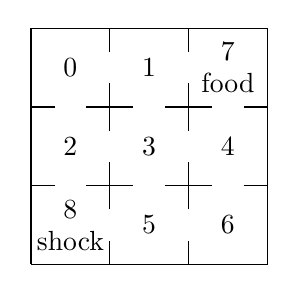
\begin{tikzpicture}
		\draw (0,0)--(3,0)--(3,3)--(0,3)--(0,0);
		\draw (1,0)--(1,0.3) (1,0.7)--(1,1.3) (1,1.7)--(1,2.3) (1,2.7)--(1,3);
		\draw (2,0)--(2,0.3) (2,0.7)--(2,1.3) (2,1.7)--(2,2.3) (2,2.7)--(2,3);
		\draw (0,1)--(0.3,1) (0.7,1)--(1.3,1) (1.7,1)--(2.3,1) (2.7,1)--(3,1);
		\draw (0,2)--(0.3,2) (0.7,2)--(1.3,2) (1.7,2)--(2.3,2) (2.7,2)--(3,2);
		\draw (0.5,2.5)node[]{0} (1.5,2.5)node[]{1} (2.5,2.7)node[]{7} (2.5,2.3)node[]{food};
		\draw (0.5,1.5)node[]{2} (1.5,1.5)node[]{3} (2.5,1.5)node[]{4};
		\draw (0.5,0.7)node[]{8} (0.5,0.3)node[]{shock} (1.5,0.5)node[]{5} (2.5,0.5)node[]{6};
	\end{tikzpicture}
\end{figure}
\end{problem}
\begin{solution}
	\[
		\bm{P} =
		\bordermatrix{
			~ & 0 & 1 & 2 & 3 & 4 & 5 & 6 & 7 & 8 \cr
			0 & 0 & \frac{1}{2} & \frac{1}{2} & 0 & 0 & 0 & 0 & 0 & 0 \cr
			1 & \frac{1}{3} & 0 & 0 & \frac{1}{3} & 0 & 0 & 0 & \frac{1}{3} & 0 \cr
			2 & \frac{1}{3} & 0 & 0 & \frac{1}{3} & 0 & 0 & 0 & 0 & \frac{1}{3}\cr
			3 & 0 & \frac{1}{4} & \frac{1}{4} & 0 & \frac{1}{4} & \frac{1}{4} & 0 & 0 & 0 \cr
			4 & 0 & 0 & 0 & \frac{1}{3} & 0 & 0 &\frac{1}{3} & \frac{1}{3} & 0 \cr
			5 & 0 & 0 & 0 & \frac{1}{3} & 0 & 0 &\frac{1}{3} & 0 & \frac{1}{3} \cr
			6 & 0 & 0 & 0 & 0 & \frac{1}{2} & \frac{1}{2} & 0 & 0 & 0 \cr
			7 & 0 & 0 & 0 & 0 & 0 & 0 & 0 & 1 & 0 \cr
			8 & 0 & 0 & 0 & 0 & 0 & 0 & 0 & 0 & 1 \cr}
	\]
	设$u_k$为家鼠从$k$出发在遭到电击前能找到食物的概率, 显然$u_7 = 1, u_8 = 0$\\
	设$T$为进入吸收态时刻, 则当$0 \leqslant k \leqslant 6$时,
	\begin{align*}
		u_k & = \p\{X_T = 7 | X_0 = k\}                                    \\
		    & = \sum^8_{i=0}\p\{X_T = 7, X_1 = i | X_0 = k\}               \\
		    & = \sum^8_{i=0}\p\{X_T = 7, X_1 = i\} \p\{X_1 = i | X_0 = k\}
	\end{align*}
	\[\therefore
		\begin{cases}
			u_0 = \frac{1}{2}(u_1+u_2)         \\
			u_1 = \frac{1}{3}(u_0+u_3+u_7)     \\
			u_2 = \frac{1}{3}(u_0+u_3+u_8)     \\
			u_3 = \frac{1}{4}(u_1+u_2+u_4+u_5) \\
			u_4 = \frac{1}{3}(u_3+u_6+u_7)     \\
			u_5 = \frac{1}{3}(u_3+u_6+u_8)     \\
			u_6 = \frac{1}{2}(u_4+u_5)         \\
			u_7 = 1                            \\
			u_8 = 0
		\end{cases}\Rightarrow
		\begin{cases}
			u_0 = \frac{1}{2} \\
			u_1 = \frac{2}{3} \\
			u_2 = \frac{1}{3} \\
			u_3 = \frac{1}{2} \\
			u_4 = \frac{2}{3} \\
			u_5 = \frac{1}{3} \\
			u_6 = \frac{1}{2} \\
			u_7 = 1           \\
			u_8 = 0
		\end{cases}
	\]
\end{solution}

\begin{problem}{3.7}
记$Z_i,i=1,2,\cdots$为一串独立同分布的离散随机变量.$\p\{Z_i=k\}=p_k \geqslant 0,k=0,1,2,\cdots,\quad \sum\limits^\infty_{k=0}p_k = 1$.记$X_n = Z_n, n = 1, 2, \cdots$.试求过程$X_n$的转移概率矩阵.
\end{problem}
\begin{solution}
	$\because \p\{X_{n+1} = i_{n+1} | X_1 = i_1, \cdots , X_n = i_n\} = \p\{X_{n+1} = i_{n+1}\}$\\
	$\p\{X_{n+1} = i_{n+1} | X_n = i_n\} = \p\{X_{n+1} = i_{n+1}\}$\\
	$\therefore \p\{X_{n+1} = i_{n+1} | X_1 = i_1, \cdots , X_n = i_n\} = \p\{X_{n+1} = i_{n+1} | X_n = i_n\}$\\
	$\therefore \{X_n\}$是一M.C.,其转移概率矩阵为
	\[\bm{P} =
		\begin{pmatrix}
			p_0    & p_1    & p_2    & \cdots \\
			p_0    & p_1    & p_2    & \cdots \\
			p_0    & p_1    & p_2    & \cdots \\
			\vdots & \vdots & \vdots & \ddots
		\end{pmatrix}\]
\end{solution}

\begin{problem}{3.8}
对第7题中的$Z_i$, 令$X_n = \max \{Z_1, \cdots , Z_n\}, n = 1, 2, \cdots$, 并约定$X_0 = 0$. $X_n$是否为Markov链? 如果是, 其转移概率阵是什么?
\end{problem}
\begin{solution}
	\begin{align*}
		X_{n+1} & = \max \{Z_1, \cdots, Z_n, Z_{n+1}\}         \\
		        & = \max \{\max\{Z_1, \cdots, Z_n\}, Z_{n+1}\} \\
		        & = \max \{X_n, Z_{n+1}\}
	\end{align*}
	$\therefore \{X_n\}$是M.C.
	\[
		P_{ij} =
		\begin{cases}
			0                      & , j < i     \\
			p_j                    & , j > i     \\
			\sum\limits^i_{k=0}p_k & , j = i     \\
			0                      & , \text{其他}
		\end{cases}
	\]
	其转移概率矩阵为
	\[
		\bm{P} =
		\begin{pmatrix}
			p_0    & p_1     & p_2         & \cdots \\
			0      & p_0+p_1 & p_2         & \cdots \\
			0      & 0       & p_0+p_1+p_2 & \cdots \\
			\vdots & \vdots  & \vdots      & \ddots
		\end{pmatrix}
	\]
\end{solution}

\begin{problem}{3.9}
设$f^{(n)}_{ij}$表示从$i$出发在$n$步转移时首次到达$j$的概率, 试证明
\[P^{(n)}_{ij} = \sum^n_{k=0}f^{(k)}_{ij}P^{(n-k)}_{jj}.\]
\end{problem}
\begin{solution}[1]
	设$T_j = \min \{n: n \geqslant 0 \,\text{且}\, X_n = j\}$
	\[\begin{split}
			\therefore P^{(n)}_{ij} & = \p\{X_n = j | X_0 = i\} = \sum^n_{k=0}\p\{X_n = j, T_j = k | X_0 = i\}\\
			& = \sum^n_{k=0}\p\{T_j = k | X_0 = i\}P^{(n-k)}_{jj}\\
			& = \sum^n_{k=0}\p\{X_k = j, X_s\neq j(s = 0,1,\cdots, k-1) | X_0 = i\}P^{(n-k)}_{jj}\\
			& = \sum^n_{k=0}f^{(k)}_{ij} P^{(n-k)}_{jj}
		\end{split}\]
\end{solution}
\begin{solution}[2(郑老师解法)]
	\[\begin{aligned}
			  & P_{ij}^{(n)}=\p\{X_n=j|X_0=i\}                                                                                                                                                             \\
			= & \p\{\underbrace{X_n=j}_{\color{red}C},\underbrace{X_1=j}_{\color{red}B}|\underbrace{X_0=i}_{\color{red}A}\} + \p\{X_n=j,X_1\neq j|X_0=i\}\xlongequal{\color{red}\p(BC|A)=\p(B|A)\p(C|AB)}  \\
			= & \p\{X_n=j|X_0=i,X_1=j\}P_{ij} + \p\{X_n=j,X_1\neq j|X_0=i\}                                                                                                                                \\
			= & f_{ij}^{(1)}P_{jj}^{(n-1)} + \p\{X_n=j,X_1\neq j|X_0=i\}                                                                                                                                   \\
			= & f_{ij}^{(1)}P_{jj}^{(n-1)} + \p\{\underbrace{X_n=i}_{\color{red}C},\underbrace{X_2=j,X_1\neq j}_{\color{red}B}|\underbrace{X_0=i}_{\color{red}A}\} + \p\{X_n=j,X_2\neq j,X_1\neq j|X_0=i\} \\
			= & f_{ij}^{(1)}P_{jj}^{(n-1)} + \p\{X_2=j,X_1\neq j|X_0=i\}\p\{X_n=j|X_0=i,X_1\neq j,X_2=j\}                                                                                                  \\
			  & +\p\{X_n=j,X_2\neq j,X_1\neq j|X_0=i\}                                                                                                                                                     \\
			= & f_{ij}^{(1)}P_{jj}^{(n-1)} + f_{ij}^{(2)}P_{jj}^{(n-2)} + \p\{X_n=j,X_2\neq j,X_1\neq j|X_0=i\} = \cdots                                                                                   \\
			= & \sum_{k=1}^{n-1}f_{ij}^{(k)}P_{jj}^{(n-k)} + \p\{X_n=j,X_k\neq j,k=1,2,\dots , n-1|X_0=i\}                                                                                                 \\
			= & \sum_{k=1}^{n-1}f_{ij}^{(k)}P_{jj}^{(n-k)} + f_{ij}^{(n)}P_{jj}^{(0)}                                                                                                                      \\
			= & \sum_{k=1}^{n}f_{ij}^{(k)}P_{jj}^{(n-k)}
		\end{aligned}\]
\end{solution}

\begin{problem}{3.10}
对第7题中的$Z_i$, 若定义$X_n = \sum\limits^n_{i=1}Z_i, n = 1, 2, \cdots, X_0 = 0$, 试证$X_n$为Markov链. 并求其转移概率矩阵.
\end{problem}
\begin{solution}
	对$n \geqslant 0$有
	\[\begin{split}
			& \quad \p\{X_{n+1} = i_{n+1} | X_0 = i_0, \cdots, X_n = i_n\} \qquad (i_0 = 0)\\
			& = \p\{Z_{n+1} = i_{n+1} - i_n | X_0 = i_0, \cdots, X_n = i_n\}\\
			& = \p\{Z_{n+1} = i_{n+1} - i_n\}\\
			& = \begin{cases}
				P_{i_{n+1}-i_n} & , i_{n+1} - i_n = 0,1,2,\cdots \\
				0               & , ow
			\end{cases}
		\end{split}\]
	\[\begin{split}
			& \{X_{n+1} = i_{n+1} | X_n = i_n\}\\
			= & \p\{X_{n} + Z_{n+1} = i_{n+1} | X_n = i_n\}\\
			= & \p\{Z_{n+1} = i_{n+1} - i_n\}
		\end{split}\]
	$\therefore X_n $是M.C.
	\[\bm{P} =
		\begin{pmatrix}
			p_0    & p_1    & p_2    & \cdots \\
			0      & p_0    & p_1    & \cdots \\
			0      & 0      & p_0    & \cdots \\
			\vdots & \vdots & \vdots & \ddots
		\end{pmatrix}
	\]
\end{solution}

\begin{problem}{3.11}
一Markov链有状态$0,1,2,3$和转移概率矩阵
\[
	\bm{P} =
	\begin{pmatrix}
		0           & \frac{1}{2} & 0 & \frac{1}{2} \\
		0           & 0           & 1 & 0           \\
		0           & 0           & 0 & 1           \\
		\frac{1}{2} & 0           & 0 & \frac{1}{2}
	\end{pmatrix}
\]
试求$f^{(n)}_{00}, n = 1,2,3,4,5,\cdots, $ 其中$f^{(n)}_{00}$由
\[\p\{X_n = i, X_k \neq i, k = 1, \cdots, n-1 | X_0 = i\}\]定义.
\end{problem}
\begin{solution}
	$f^{(1)}_{00} = P_{00} = 0,\quad f^{(2)}_{00} = \begin{pmatrix}\frac{1}{2} & 0 & \frac{1}{2}\end{pmatrix}\begin{pmatrix}0 & 0 & \frac{1}{2}\end{pmatrix}^T = \frac{1}{4}$ \\
	对$n \geqslant 2$有
	\[f^{(n)}_{00} =
		\begin{pmatrix}\frac{1}{2} & 0 & \frac{1}{2}\end{pmatrix}
		\begin{pmatrix}
			0 & 1 & 0           \\
			0 & 0 & 1           \\
			0 & 0 & \frac{1}{2} \\
		\end{pmatrix}^{n-2}
		\begin{pmatrix}0 \\ 0 \\ \frac{1}{2}\end{pmatrix}
	\]
	当$n=3$时, $f^{(3)}_{00} = \frac{1}{8}$\\
	当$n \geqslant 4$时,
	\[f^{(n)}_{00} =
		\begin{pmatrix}\frac{1}{2} & 0 & \frac{1}{2}\end{pmatrix}
		\begin{pmatrix}
			0 & 0 & \frac{1}{2^{n-2}} \\
			0 & 0 & \frac{1}{2^{n-1}} \\
			0 & 0 & \frac{1}{2^{n-1}}
		\end{pmatrix}
		\begin{pmatrix}0 \\ 0 \\ \frac{1}{2}\end{pmatrix}
		= \frac{1}{2^n} + \frac{1}{2^{n+2}}
	\]
\end{solution}

\begin{problem}{3.12}
在成败型的重复试验中, 每次试验结果为成功(S)或失败(F). 同一结果相继出现称为一个游程(run), 比如一结果$FSSFFFSF$中共有两个成功游程, 三个失败游程. 设成功概率为$p$, 失败概率为$q = 1 - p$. 记$X_n$为第$n$次试验后成功游程的长度(若第$n$次试验, 则$X_n = 0$). 试证$\{X_n, n = 1,2,\cdots\}$为一Markov链, 并确定其转移概率阵. 记$T$为返回状态$0$的时间, 试求$T$的分布及均值. 并由此对这一Markov链的状态进行分类.
\end{problem}
\begin{solution}
	$X_{n+1} =
		\begin{cases}
			X_{n+1} & , \text{第$n+1$次试验成功} \\
			0       & , \text{第$n+1$次试验失败} \\
		\end{cases}\Rightarrow \{X_n\}\text{是M.C.}$.
	$\p(X_{n+1} = j | X_n = i) =
		\begin{cases}
			p, j = i + 1 \\
			q, j = 0
		\end{cases}$
	\[\bm{P} =
		\bordermatrix{
			~ & 0 & 1 & 2 & 3 & \cdots \cr
			0 & q & p & 0 & 0 & \cdots \cr
			1 & q & 0 & p & 0 & \cdots \cr
			2 & q & 0 & 0 & p & \cdots \cr
			\vdots & \vdots & \vdots & \vdots & \vdots & \ddots \cr}
	\]
	$T = \min \{n : X_n = 0, X_s \neq 0 \quad (s = 1,2,\cdots, n-1)\}$\\
	$\p(T = k) = p^{k-1} q \qquad (k=1,2,\cdots)$\\
	$\E(T) = \sum^{\infty}_{k=1}p^{k-1} qk$\quad $\therefore p\E(T) = \sum^{\infty}_{k=1}p^k qk$\\
	$\therefore (1-p)\E(T) = q\E(T) = q + pq + p^2 q + \cdots = \frac{q}{1-p} = 1$\\
	$\therefore \E(T) = \frac{1}{q} = \frac{1}{1-p} = \mu_0$,故所有状态互通,为一类
	\\ 又$\sum_{k=1}^{\infty}f_{00}^{(k)} = \sum_{k=1}^{\infty}p^{k-1}q = 1 = f_{00}$,故0为常返,且为正常返($\mu_0=\frac{1}{1-p}$).故本M.C.为不可约遍历的.
	\\ (或者由$\bm{\pi}=\bm{\pi}\bm{P}$及$\sum_{j=0}^{\infty}\pi _j=1$解出其平稳分布为:
	$\pi = \{\pi _n,n\geqslant 0\} = \{q,pq,pq^2,\cdots ,p^nq,\cdots \}$)由此判断M.C.为正常返
	\begin{figure}[H]
		\centering
		\begin{tikzpicture}
			[%%%%%%%%%%%%%%%%%%%%%%%%%%%%%%%%%%%%%%%%%%%%%%%%%%%%%%%%%%
				node distance =.8cm,>=Stealth,
				place/.style={circle,draw=blue!50,fill=blue!20,thick,
						inner sep=0pt,minimum size=6mm},
				dotsstyle/.style={text=blue}
			]%%%%%%%%%%%%%%%%%%%%%%%%%%%%%%%%%%%%%%%%%%%%%%%%%%%%%%%%%%
			\node[place] (0) {$0$};
			\node[place] (1) [right=of 0] {$1$};
			\node[place] (2) [right=of 1] {$2$};
			\node[place] (3) [right=of 2] {$3$};
			\node[place] (4) [right=of 3] {$4$};
			\node[dotsstyle] (dots1) [node distance=0.5cm,right=of 4] {$\cdots $};
			\node[place] (k) [node distance=0.5cm,right=of dots1] {$k$};
			\node[dotsstyle] (dots2) [node distance=0.5cm,right= of k] {$\cdots $};

			\draw [->,thick] (0.south west) arc (-45:-315:0.3) node [above left] {$q$};

			\foreach \i in {0,1,2,3}
			\draw [->,thick] (\i.east) to node[above] {$p$}({\the\numexpr\i+1}.west);

			\draw [->,thick] (4.east) to node[above] {$p$} (dots1.west);
			\draw [->,thick] (dots1.east) to node[above] {$p$} (k.west);
			\draw [->,thick] (k.east) to node[above] {$p$} (dots2.west);

			\foreach \i in {1,2,3,4}
			\draw [->,thick] (\i.south) to [bend left=45] node[above] {$q$} (0.south);

			\draw [->,thick] (k.south) to [bend left=45] node[above] {$q$} (0.south);
		\end{tikzpicture}
		\caption{3.12图解}
	\end{figure}
\end{solution}

\begin{problem}{3.13}
试证各方向游动的概率相等的对称随机游动在二维时是常返的, 而在三维时却是瞬过的.
\\ (此处答案仅给出二维情况,三维情况不是作业要求(逃))
\end{problem}
\begin{solution}[1(jkadbear及郑老师解法)]
	设$\{X_n,n\geqslant 0\}$为二维对称随机游动,其状态空间为二维实平面上所有的整数点(格点),易知该M.C.为不可约的,故仅需考虑状态0(原点$(0,0)$)的常返性,且仅需考虑$P_{00}^{(2n)}$.
	\[\begin{split}
			P_{00}^{(2n)} & = \sum_{k=0}^{n}\frac{(2n)!}{k!k!(n-k)!(n-k)!}\left(\frac{1}{4}\right)^{2n} = \left(\frac{1}{4}\right)^{2n}\sum_{k=0}^{n}\binom{2n}{n}\binom{n}{k}^{2} \\
			& = \left(\frac{1}{4}\right)^{2n}\binom{2n}{n}\underbrace{\sum_{k=0}^{n}\binom{n}{k}\binom{n}{n-k}}_{=\binom{2n}{n}}\\
			& = \left(\frac{1}{4}\right)^{2n}\binom{2n}{n}^{2} = \left(\frac{1}{4}\right)^{2n}\left[\frac{(2n)!}{(n!)^2}\right]^2 \xrightarrow{\text{Stirling}}\left(\frac{1}{4}\right)^{2n}\left[\frac{(2n)^{2n+\frac{1}{2}}\e^{-2n}\sqrt{2\uppi}}{n^{2n+1}\e^{-2n}2\uppi}\right]^2\\
			& = \frac{1}{n\uppi}
		\end{split}\]
	而级数$\sum_{n=1}^{\infty}\frac{1}{n\uppi}$发散,故$\sum_{n=1}^{\infty}P_{00}^{(n)}$发散,从而该M.C.为常返的.进一步可以证明$\{X_n,n\geqslant 0\}$为零常返的,且周期为2
\end{solution}
\begin{solution}[2]
	前面大差不差.
	\[\begin{split}
			P_{ii}^{(n)} & = \sum_{k=0}^{n}\binom{2n}{k,k,n-k,n-k}\left(\frac{1}{4}\right)^{2n} = \sum_{k=0}^{n}\frac{(2n)!}{k!k!(n-k)!(n-k)!}\frac{1}{2^{4n}} \\
			& = \sum_{k=0}^{n}\binom{n}{k}\frac{(n+1)\cdots (2n)}{k!(n-k)!}\frac{1}{2^{4n}} = \sum_{k=0}^{n}\binom{n}{k}\frac{(\frac{n+1}{2})(\frac{n+2}{2})\cdots n}{k!(n-k)!}\cdot \frac{1}{2^{3n}}\\
			& > \sum_{k=0}^{n}\binom{n}{k}\frac{n!}{k!(n-k)!}\cdot \frac{1}{2^{3n}}\\
			& =\sum_{k=0}^{n}\binom{n}{k}^{2}\cdot \frac{1}{2^{3n}} > \sum_{k=0}^{n}\binom{n}{k}\cdot \frac{1}{2^{3n}} >\sum_{k=0}^{n}\binom{n}{k}\frac{1}{2^n} = 1
		\end{split}\]
	$\therefore \sum_{n=1}^{\infty}P_{ii}^{(n)}>\sum_{n=1}^{\infty}1 = +\infty \Rightarrow i$为常返的,又因为二维随机游动任意状态互达,故该Markov链常返
\end{solution}

\begin{problem}{3.14}
某厂对该厂生产的同类产品的三种型号调查顾客的消费习惯. 并把它们归结为Markov链模型. 记顾客消费习惯在 $A, B, C $ 三种型号间的转移概率矩阵分别为下列四种. 请依这些转移阵所提供的信息对厂家提出关于 $A, B$ 两种型号的咨询意见.
\[
	\begin{split}
		&(1)\begin{pmatrix}
			1 & 0 & 0 \\
			0 & 1 & 0 \\
			0 & 0 & 0
		\end{pmatrix},\qquad
		(2)\begin{pmatrix}
			0           & \frac{1}{2} & \frac{1}{2} \\
			\frac{1}{2} & 0           & \frac{1}{2} \\
			\frac{1}{2} & \frac{1}{2} & 0
		\end{pmatrix},\\[0.5cm]
		&(3)\begin{pmatrix}
			\frac{1}{2} & 0           & \frac{1}{2} \\
			\frac{1}{3} & \frac{1}{3} & \frac{1}{3} \\
			\frac{1}{2} & 0           & \frac{1}{2}
		\end{pmatrix},\qquad
		(4)\begin{pmatrix}
			0 & 1 & 0 \\
			0 & 0 & 1 \\
			1 & 0 & 0
		\end{pmatrix}.
	\end{split}
\]
\end{problem}
\begin{solution}
	\begin{enumerate}[label=(\arabic*)]
		\item \begin{enumerate}[label=(\alph*)]
			      \item 不是概率转移矩阵, 第三行行和不为$1$.
			      \item 郑老师的作业题将此图改为
			            $\bm{P}=
				            \begin{pmatrix}
					            1 & 0 & 0 \\
					            0 & 1 & 0 \\
					            0 & 0 & 1
				            \end{pmatrix}$
			            相应的解答为:$A,B,C$三个状态均为常返,且均为吸收态,但相互之间不可达.说明三种产品都比较好,顾客流都很稳定,但A与B谁更好一些无法比较;
		      \end{enumerate}
		\item \[
			      \bm{P}^2 =
			      \begin{pmatrix}
				      0           & \frac{1}{2} & \frac{1}{2} \\
				      \frac{1}{2} & 0           & \frac{1}{2} \\
				      \frac{1}{2} & \frac{1}{2} & 0
			      \end{pmatrix}^2 =
			      \begin{pmatrix}
				      \frac{1}{2} & \frac{1}{4} & \frac{1}{4} \\
				      \frac{1}{4} & \frac{1}{2} & \frac{1}{4} \\
				      \frac{1}{4} & \frac{1}{4} & \frac{1}{2} \\
			      \end{pmatrix}
		      \]
		      $\therefore A,B,C$三状态互通, 所有状态可遍历.\\
		      设$\bm{\pi}=(\pi_A,\pi_B,\pi_C)$为经过长时间后三个产品的市场占有额,则
		      \[
			      \begin{cases}
				      (\pi_A,\pi_B,\pi_C)
				      \begin{pmatrix}
					      0           & \frac{1}{2} & \frac{1}{2} \\
					      \frac{1}{2} & 0           & \frac{1}{2} \\
					      \frac{1}{2} & \frac{1}{2} & 0
				      \end{pmatrix} = (\pi_A,\pi_B,\pi_C) \\
				      \pi_A+\pi_B+\pi_C = 1
			      \end{cases} \Rightarrow
			      \pi_A = \pi_B = \pi_C = \frac{1}{3}
		      \]
		      $\therefore$三个品牌竞争力差不多, 可以都生产.但从转移概率矩阵来看,$A,B$都有需要改进之处
		\item 由归纳法可知
		      \[
			      \bm{P}^n=
			      \begin{pmatrix}
				      \frac{1}{2}                          & 0             & \frac{1}{2}                          \\
				      \frac{1}{2}\big(1-\frac{1}{3^n}\big) & \frac{1}{3^n} & \frac{1}{2}\big(1-\frac{1}{3^n}\big) \\
				      \frac{1}{2}                          & 0             & \frac{1}{2}
			      \end{pmatrix}
		      \]
		      可见
		      \[\pi_B = \lim_{n\to \infty} \Big(\frac{1}{3}\Big)^n = 0,\]
		      \[
			      \begin{cases}
				      (\pi_A, \pi_C)\cdot
				      \begin{pmatrix}
					      \frac{1}{2} & \frac{1}{2} \\
					      \frac{1}{2} & \frac{1}{2}
				      \end{pmatrix} = (\pi_A, \pi_C) \\
				      \pi_A + \pi_C = 1
			      \end{cases} \Rightarrow
			      \pi_A = \pi_C = \frac{1}{2}
		      \]
		      $\therefore B$将逐渐淡出市场, 建议停止生产$B$, 扩大对$A$的生产.$A,C$常返,$B$瞬过.$A,B$比较,顾客更倾向于消费$A$,且从长远观点看,顾客消费$B$的可能性将趋于零,市场将由$A,C$二分天下.
		\item $\therefore A,B,C$三状态互通, 所有状态可遍历.
		      \[
			      \begin{cases}
				      (\pi_A,\pi_B,\pi_C)
				      \begin{pmatrix}
					      0 & 1 & 0 \\
					      0 & 0 & 1 \\
					      1 & 0 & 0
				      \end{pmatrix} = (\pi_A,\pi_B,\pi_C) \\
				      \pi_A+\pi_B+\pi_C = 1
			      \end{cases} \Rightarrow
			      \pi_A = \pi_B = \pi_C = \frac{1}{3}
		      \]
		      $\therefore A,B,C$市场占有率相同, 可维持现状.与(2)同
		      \begin{figure}[H]
			      \centering
			      \begin{tikzpicture}
				      [%%%%%%%%%%%%%%%%%%%%%%%%%%%%%%%%%%%%%%%%%%%%%%%%%%%%%%%%%%
					      node distance =.8cm,>=Stealth,
					      place/.style={circle,draw=blue!50,fill=blue!20,thick,
							      inner sep=0pt,minimum size=6mm},
					      dotsstyle/.style={text=blue}
				      ]%%%%%%%%%%%%%%%%%%%%%%%%%%%%%%%%%%%%%%%%%%%%%%%%%%%%%%%%%%
				      \node[place] (A) {$A$};
				      \node[place] (B) [below left=of A] {$B$};
				      \node[place] (C) [below right=of A] {$C$};

				      \draw[->,thick] (A.south west) to node[above]{1} (B.north east);
				      \draw[->,thick] (B.east) to node[above]{1} (C.west);
				      \draw[->,thick] (C.north west) to node[above]{1} (A.south east);
			      \end{tikzpicture}
			      \caption{3.14(4)图解}
		      \end{figure}
	\end{enumerate}
\end{solution}

\begin{problem}{3.15}
考虑一有限状态的Markov链. 试证明
\begin{enumerate}[label=(\alph*)]
	\item 至少有一个状态是常返的
	\item 任何常返状态必定是正常返的.
\end{enumerate}
\end{problem}
\begin{solution}[1]
	\begin{enumerate}[label=(\alph*)]
		\item 反设所有状态均为瞬过或零常返(加强结论),则对$\forall i \in S$, 有
		      \begin{equation}
			      \lim_{n\to +\infty} P^{(n)}_{ii} = 0 \label{eq3.15.1}
		      \end{equation}
		      考虑$P^{(n)}_{ij} = \sum\limits^{+\infty}_{k=1} f^{(k)}_{ij} P^{(n-k)}_{jj}$, 则有
		      \begin{equation}
			      \sum^\ell_{k=1} f^{(k)}_{ij} P^{(n-k)}_{jj} \leqslant P^{(n)}_{ij} \leqslant \sum^\ell_{k=1} f^{(k)}_{ij} P^{(n-k)}_{jj} + \sum^{+\infty}_{k=l} f^{(k)}_{ij} \label{eq3.15.2}
		      \end{equation}
		      固定$\ell$, 令$n\to +\infty$, 则由 \eqref{eq3.15.1} 得
		      \begin{equation}
			      0 \leqslant \lim_{n\to +\infty} P^{(n)}_{ij} \leqslant 0 + \sum^{+\infty}_{k=\ell} f^{(k)}_{ij} \label{eq3.15.3}
		      \end{equation}
		      在 \eqref{eq3.15.3} 中令$\ell \to +\infty$, 由于$\sum\limits^{\infty}_{k=1} f^{(k)}_{ij} \leqslant 1$收敛
		      \begin{equation}
			      \therefore \lim_{n\to +\infty} P^{(n)}_{ij} = 0 \label{eq3.15.4}
		      \end{equation}
		      若此有限状态M.C.有$N$个状态, 则
		      \begin{equation}\sum^{N}_{j=1} P^{(n)}_{ij} = 1 \label{eq3.15.5}
		      \end{equation}
		      \eqref{eq3.15.5} 中令$n\to +\infty$, 由 \eqref{eq3.15.4} 得$0=1$, 矛盾$\Rightarrow$至少有一个状态是(正)常返的
		\item 若存在零常返状态$i$, 可构造$C(i) = \{j|i\leftrightarrow j\}$,
		      则$C(i)$为原M.C.的一不可约子M.C.(有限状态),
		      于是$C(i)$中所有状态均为零常返, 与有限状态M.C.至少有一个正常返状态矛盾,\\
		      $\therefore$任何常返状态均为正常返
	\end{enumerate}
\end{solution}
\begin{solution}[2(郑老师解法)]
	\begin{enumerate}[label=(\alph*)]
		\item 设M.C.的状态空间为$S=\{0,1,2,\cdots ,N\}$.(反证法)若命题为真,则M.C.的所有状态为瞬过的.从而对$\forall i,j\in S$有$\lim_{n \to \infty}P_{ij}^{(n)}=0$,但另一方面又有:
		      \[\sum_{j=0}^{N}P_{ij}^{(n)}=1\qquad (\forall i\in S,n\in \mathbb{N})\]
		      两边取极限得到
		      \[1=\lim_{n \to \infty}\sum_{j=0}^{N}P_{ij}^{(n)} = \sum_{j=0}^{N}\lim_{n \to \infty}P_{ij}^{(n)} = \sum_{j=0}^{N}0 = 0\]
		      矛盾.从而(a)得证
		\item (反证法)若命题不真,则M.C.至少存在一个零常返状态.设$S_1\subseteq S$为全体零常返状态构成的子集,易证$S_1$为闭集.为叙述方便,无妨设$S_1=\{0,1,2,\cdots ,M\}\quad (M\leqslant N)$.则原M.C.限制在$S_1$上仍为一M.C.,从而有:
		      \begin{equation}
			      \sum_{j\in S_1}P_{ij}[w(n)] = \sum_{j=0}^{M}P_{ij}^{(n)} = 1 \qquad (\forall i\in S_1,n\in \mathbb{N}) \label{eq3.15b}
		      \end{equation}
		      另一方面,由类似于$(a)$的理由可知,对于$\forall i,j\in S_1$,有$\lim_{n \to \infty}P_{ij}^{(n)} = 0$,从而对 \eqref {eq3.15b} 式两边取极限得到:
		      \[0 = \lim_{n \to \infty}\sum_{j=1}^{M}P_{ij}^{(n)} = \lim_{n \to \infty}1 = 1\]
		      矛盾.从而该M.C.不可能存在零常返状态.即(b)得证.$\qedhere$
	\end{enumerate}
\end{solution}

\begin{problem}{3.16}
考虑一生长与灾害模型. 这类Markov链有状态 $0,1,2,\cdots,$ 当过程处于状态$i$时它既可能以概率$p_i$转移到$i+1$(生长)也能以概率$q_i = 1 - p_i$ 落回到状态$0$(灾害). 而从状态“0”又必然“无中”生有. 即$P_{01} \equiv 1$.
\begin{enumerate}[label=(\alph*)]
	\item 试证所有状态为常返的条件是\[\lim_{n\to \infty}(p_1p_2p_3\cdots p_n) = 0.\]
	\item 若此链为常返, 试求其为零常返的条件.
\end{enumerate}
\end{problem}
\begin{solution}[1]
	\begin{enumerate}[label=(\alph*)]
		\item 其概率转移阵为
		      \[
			      \bm{P} =
			      \bordermatrix{
				      ~ & 0   & 1 & 2   & 3   & \cdots \cr
				      0 & 0   & 1 & 0   & 0   & \cdots \cr
				      1 & q_1 & 0 & p_1 & 0   & ~ \cr
				      2 & q_2 & 0 & 0   & p_2 & ~ \cr
				      3 & q_3 & 0 & 0   & 0 ~ \cr
				      \vdots & \vdots & ~ & ~ & ~ & \ddots \cr
			      }
		      \]
		      易知此M.C.不可约, $\therefore$只需证状态$0$常返$\Leftrightarrow~\lim\limits_{n\to +\infty}p_1 p_2\cdots p_n = 0$\\
		      显然$f^{(0)}_{00} = f^{(1)}_{00} = 0, f^{(2)}_{00} = q_1$
		      \[
			      \begin{split}
				      f_{00}^{(n)} & =
				      \begin{pmatrix}
					      1 & 0 & 0 & \cdots
				      \end{pmatrix}
				      \begin{pmatrix}
					      0      & p_1    & 0      & 0      & \cdots \\
					      0      & 0      & p_2    & 0      & \cdots \\
					      0      & 0      & 0      & p_3    & \cdots \\
					      \vdots & \vdots & \vdots & \vdots & \ddots
				      \end{pmatrix}^{n-2}
				      \begin{pmatrix}
					      q_1 \\
					      q_2 \\
					      q_3 \\
					      \vdots
				      \end{pmatrix}\\
				      & = \bm{A}\bm{B}^{n-2}\bm{C}^T, \quad (n\geqslant 3)
			      \end{split}
		      \]
		      易知
		      \[
			      \bm{B}^{n-2} =
			      \begin{pmatrix}
				      \underbrace{\begin{matrix}0 & \cdots & 0 \end{matrix}}_{n-2\text{个}} & p_1\cdots p_{n-2} & 0                 & \cdots \\
				      \underbrace{\begin{matrix}0 & \cdots & 0 \end{matrix}}_{n-2\text{个}} & 0                 & p_2\cdots p_{n-2} & \cdots \\
				      \vdots                                                               & \vdots            & \vdots            & \ddots
			      \end{pmatrix}
		      \]
		      \[\therefore f^{(n)}_{00} = (\,\overbrace{0\,\cdots\,0}^{n-2\text{个}}\,p_1\cdots p_{n-2}\,0\,0\,\cdots)(q_1\,q_2\,\cdots)^T = p_1\cdots p_{n-2}q_{n-1}\]
		      \[
			      \begin{split}
				      \therefore f_{00} & = q_1 + \sum^{+\infty}_{n=3}p_1\cdots p_{n-2}q_{n-1}\\
				      & = 1 - p_1 + \sum^{+\infty}_{n=3}(p_1\cdots p_{n-2} - p_1\cdots p_{n-2}p_{n-1})\\
				      & = 1 - \lim_{n\to +\infty}p_1 p_2\cdots p_n
			      \end{split}
		      \]
		      而状态$0$常返$\Leftrightarrow f_{00} = 1 \Leftrightarrow \lim\limits_{n\to +\infty}p_1 p_2\cdots p_n = 0$.
		\item 只需考虑状态$0$,
		      \[
			      \begin{split}
				      \mu_0 & = \sum^{+\infty}_{n=0}nf^{(n)}_{00}\\
				      & = 2(1-p_1)+\sum^{+\infty}_{n=3}n(p_1\cdots p_{n-2} - p_1 \cdots p_{n-1})\\
				      & = 2 + p_1 + p_1 p_2 + p_1 p_2 p_3 + \cdots
			      \end{split}
		      \]
		      若为零常返, 则$\mu_0 = +\infty \Leftrightarrow $级数$\sum\limits^{+\infty}_{n=1}p_1\cdots p_n$发散(且通项趋于$0$)
	\end{enumerate}
\end{solution}
\begin{solution}[2(郑老师解法)]
	该M.C.的状态转移图可画出:
	\begin{figure}[H]
		\centering
		\begin{tikzpicture}
			[%%%%%%%%%%%%%%%%%%%%%%%%%%%%%%%%%%%%%%%%%%%%%%%%%%%%%%%%%%
				node distance =.8cm,>=Stealth,
				place/.style={circle,draw=blue!50,fill=blue!20,thick,
						inner sep=0pt,minimum size=6mm},
				dotsstyle/.style={text=blue}
			]%%%%%%%%%%%%%%%%%%%%%%%%%%%%%%%%%%%%%%%%%%%%%%%%%%%%%%%%%%
			\node[place] (0) {$0$};
			\node[place] (1) [right=of 0] {$1$};
			\node[place] (2) [right=of 1] {$2$};
			\node[place] (3) [right=of 2] {$3$};
			\node[place] (4) [right=of 3] {$4$};
			\node[dotsstyle] (dots1) [node distance=0.5cm,right=of 4] {$\cdots $};
			\node[place] (k) [node distance=0.05cm,right=of dots1] {$k$};
			\node[dotsstyle] (dots2) [node distance=0.5cm,right=of k] {$\cdots $};

			\foreach \i in {1,2,3}
			\draw [->,thick] (\i.east) to node[above] {$p_{\i}$}({\the\numexpr\i+1}.west);

			\draw [->,thick] (0.east) to node[above] {$p_0=1$} (1.west);


			\draw [->,thick] (4.east) to node[above] {$p_4$} (dots1.west);
			\draw [->,thick] (k.east) to node[above] {$p_{k}$} (dots2.west);

			\foreach \i in {1,2,3,4}
			\draw [->,thick] (\i.south) to [bend left=45] node[above] {$q_{\i}$} (0.south);

			\draw [->,thick] (k.south) to [bend left=45] node[above] {$q_k$} (0.south);
			\draw (dots2) node [right] {$q_i=1-p_i,i\geqslant 1,p_0=1$};
		\end{tikzpicture}
		\caption{3.16图解}
	\end{figure}
	\begin{enumerate}[label=(\alph*)]
		\item 由上图易知M.C.为不可约,非周期的.又:
		      \[f_{00}^{(1)}=0, f_{00}^{(2)}=q_1=1-p_1, f_{00}^{(3)}=p_1(1-p_2), \cdots ,f_{00}^{(n)}=p_1p_2\cdots p_{n-2}(1-p_{n-1})\]
		      从而\[f_{00}^{(n)} = \sum_{n=2}^{\infty}p_1p_2\cdots p_{n-2}(1-p_{n-1} = \lim_{n \to \infty}(1-p_1 p_2 \cdots p_n))\]
		      故0及所有状态为常返$\Longleftrightarrow \lim\limits_{n\to \infty}p_1 p_2 \cdots p_n = 0$
		\item 求解线性方程组$\displaystyle \bm{\pi} = \bm{\pi}\bm{P},\quad \sum_{j=0}^{\infty}\pi _j = 1$解得:
		      \[
			      \begin{cases}
				      \pi_1 = \pi_0         \\
				      \pi_2 = p_1 \pi_0     \\
				      \hspace{0.6cm} \vdots \\
				      \pi_n = p_1 p_2 \cdots p_{n-1}\pi_0
			      \end{cases}\quad \Rightarrow
			      \pi_0 = \frac{1}{2+\sum_{n=1}^{\infty}p_1 p_2 \cdots p_n}
			      \quad \text{故:}
		      \]
		      \begin{itemize}
			      \item 当$\sum_{n=1}^{\infty}p_1 p_2 \cdots p_n < +\infty$时,平稳分布$\bm{\pi}$存在,此时M.C.为正常返,亦即为不可约遍历.
			      \item 当$\sum_{n=1}^{\infty}p_1 p_2 \cdots p_n = +\infty$但$\lim\limits_{n\to \infty}p_1 p_2 \cdots p_n = 0$时,正常返
			      \item 当$\lim\limits_{n\to \infty}p_1 p_2 \cdots p_n = p > 0$时,M.C.为瞬过的.
		      \end{itemize}
		      亦可直接计算$\mu_0 = \sum_{n=1}^{\infty}nf_{00}^{(n)} = \sum_{n=2}^{\infty}np_1 p_2 \cdots p_{n-2}(1-p_{n-1}) = 2+\sum_{n=1}^{\infty}p_1 p_2 \cdots p_n$,从而得出同上的结论
	\end{enumerate}
\end{solution}

\begin{problem}{3.17}
试计算转移概率阵
\[
	\bm{P} =
	\begin{pmatrix}
		\frac{1}{2} & \frac{1}{2} & 0           \\
		\frac{1}{3} & \frac{1}{3} & \frac{1}{3} \\
		\frac{1}{6} & \frac{1}{2} & \frac{1}{3}
	\end{pmatrix}
\]
的极限分布.
\end{problem}
\begin{solution}
	设$\bm{\pi}$为该M.C.的平稳分布, $\bm{\pi}= (\pi_0, \pi_1, \pi_2)$\\
	\[
		\begin{cases}
			\pi \geqslant 0               \\
			\sum\limits^2_{i=0} \pi_i = 1 \\
			\bm{\pi}\bm{P} = \bm{\pi}
		\end{cases}\Rightarrow
		\bm{\pi} = \left(\frac{5}{14}, \frac{6}{14}, \frac{3}{14}\right)
	\]
	易知该M.C.不可约且遍历\quad $\therefore$ 极限分布为
	$
		\begin{pmatrix}
			\frac{5}{14} & \frac{6}{14} & \frac{3}{14} \\
			\frac{5}{14} & \frac{6}{14} & \frac{3}{14} \\
			\frac{5}{14} & \frac{6}{14} & \frac{3}{14}
		\end{pmatrix}
	$
\end{solution}

\begin{problem}{3.18}
假定在逐日的天气变化模型中, 每天的阴晴与前两天的状况关系很大. 于是可考虑$4$状态的Markov链:接连两晴天, 一晴一阴, 一阴一晴, 以及接连两阴天, 分别记为$(S, S), (S, C), (C, S), (C, C)$. 该链的转移概率阵为
\[\bm{P} =
	\bordermatrix{
		~ & (S,S) & (S,C) & (C,S) & (C,C) \cr
		(S,S) & 0.8 & 0.2 & 0 & 0 \cr
		(S,C) & 0 & 0 & 0.4 & 0.6 \cr
		(C,S) & 0.6 & 0.4 & 0 & 0 \cr
		(C,C) & 0 & 0 & 0.1 & 0.9 \cr}
\]
试求这一Markov链的平稳分布. 并求出长期平均的晴朗天数.
\end{problem}
\begin{solution}
	设其平稳分布为$\bm{\pi}= (\pi_0, \pi_1, \pi_2, \pi_3)$\\
	\[
		\begin{cases}
			\pi \geqslant 0               \\
			\sum\limits^3_{i=0} \pi_i = 1 \\
			\bm{\pi}\bm{P} = \bm{\pi}
		\end{cases} \Rightarrow
		\bm{\pi} = \left(\frac{3}{11}, \frac{1}{11}, \frac{1}{11}, \frac{6}{11}\right)
	\]
	$\bm{\pi}$反映了M.C.中各状态在长期中所占的平均比例\\
	$\therefore$一年中晴朗的天数 $ = \frac{365}{2} \times \left(\frac{3}{11} \times 2 + \frac{1}{11} + \frac{1}{11}\right) = 365\times \frac{4}{11} = 132.7$(天)
\end{solution}

\begin{problem}{3.19}
某人有$M$把伞并在办公室和家之间往返. 如某天他在家时(办公室时)下雨了而且家中(办公室)有伞他就带一把伞去上班(回家), 不下雨时他从不带伞. 如果每天与以往独立地早上(或晚上)下雨的概率为$p$, 试定义一$M+1$状态的Markov链以研究他被雨淋湿的机会.
\end{problem}
\begin{solution}
	定义$X_n$:第$n$天早晨家中雨伞数, $\therefore \{X_n, n \geqslant 0\}$为一M.C.,令$q=1-p$,可得转移概率矩阵为:
	\[
		\bm{P} =
		\bordermatrix{
			~ & 0 & 1 & 2 & \cdots & M\!-\!2 & M-1 & M \cr
			\qquad 0 & q & p & 0 & ~ & ~ & ~ & ~\cr
			\qquad 1 & pq & p^2\!+\!q^2 & pq & ~ & ~ & ~ & ~\cr
			\qquad 2 & 0 & pq & p^2\!+\!q^2 & ~ & ~ & ~ & ~\cr
			\qquad \vdots & ~ & ~ & ~ & \ddots & ~ & ~ & ~\cr
			M\!-\!1 & ~ & ~ & ~ & ~ & pq & p^2\!+\!q^2 & pq\cr
			\hspace{0.6cm} M & ~ & ~ & ~ & ~ & 0 & pq & p^2+q\cr}
	\]
	由状态转移图易知M.C.为不可约遍历的,求其平稳分布(极限分布)为:
	设$\bm{\pi}= (\pi_0, \pi_1, \cdots, \pi_M)$为其平稳分布
	\[
		\begin{cases}
			\pi_i \geqslant 0            \\
			\sum\limits^M_{i=0}\pi_i = 1 \\
			\bm{\pi}\bm{P} = \bm{\pi}
		\end{cases} \Rightarrow
		\begin{cases}
			\displaystyle \pi_0 = \frac{1-p}{M+1-p} \\
			\displaystyle \pi_i = \frac{1}{M+1-p} \quad (i = 1,2,\cdots,M)
		\end{cases}
	\]
	易知此M.C.遍历, \\
	$\therefore \pi$又是其极限分布, 其被雨淋湿的概率为
	\[
		P_{\text{淋}} = p\pi_0+p(1-p)\pi_M = 2p\frac{1-p}{M+1-p}
	\]
\end{solution}

下面几道题涉及分支过程,这部分没讲,故都没写.直接搬运刘杰班助教的习题解答\cite{刘杰班助教}.

\begin{problem}{3.20}
血液培养在时刻0从一个红细胞开始,一分钟之后红细胞死亡可能出现下面几种情况:以1/4再生2个红细胞,以1/2的概率再生1个红细胞和1个白细胞,也有1/4的概率产生2个白细胞.再过一分钟后每个红细胞以同样的规律再生下一代而白细胞则不再生.并假定每个细胞的行为是独立的.
\begin{enumerate}[label=(\alph*)]
	\item 从培养开始$n+1$分钟不出现白细胞的概率是多少?
	\item 整个培养过程停止的概率是多少?
\end{enumerate}
\end{problem}
\begin{solution}
	\begin{enumerate}[label=(\alph*)]
		\item $p=\frac{1}{4}\left(\frac{1}{4}\right)^2 \cdots \left(\frac{1}{4}\right)^{2^n}\left(\frac{1}{4}\right)^{2^{n+1}-1}$
		      \begin{itemize}
			      \item 时刻 0 1 ... $n$
			      \item 个数 1 2 ... $2^n$
		      \end{itemize}
		\item \textcolor{blue}{法一:}\\
		      \[\Phi(s) = \sum_{k=0}^{\infty}p_k s^k = \frac{1}{4}s^0 +\frac{1}{2}s^1 + \frac{1}{4}s^2\]
		      \[\Phi(s)=s\quad \frac{1}{4}s^2 - \frac{1}{2}s + \frac{1}{4} = 0\Rightarrow s=1 \Rightarrow P_{\text{消亡}}=1\]
		      \textcolor{blue}{法二:}\\
		      \[\E(Z_1)=\frac{1}{2}+2\cdot \frac{1}{4}=1=\mu \Rightarrow P_{\text{消亡}}=1\]
	\end{enumerate}
\end{solution}

\begin{problem}{3.21}
分支过程中一个体产生后代的分布为$p_0=q,p_1=p \quad (p+q=1)$,试求第$n$代总体的均值和方差及群体消亡的概率.如产生后代的分布为$p_0=1/8,p_1=1/2,p_2=1/4,p_3=1/8$,试回答同样的问题.
\end{problem}
\begin{solution}
	\begin{enumerate}[label=(\roman*)]
		\item $p_0=q, p_1=p$\\
		      $Z_1$为第1代第1个个体的后代,$\p(Z_1=k)=p_k, \E(Z_1)=\mu, \var(Z_1)=\sigma ^2$
		      \[\begin{split}
				      \E(X_{n+1}) &= \mu ^{n+1}\\
				      \var(X_{n+1}) &= \begin{cases}
					      \sigma ^2 \mu ^n \frac{1-\mu ^{n+1}}{1-\mu}, & \mu \neq 1 \\
					      (n+1)\sigma ^2,                              & \mu = 1
				      \end{cases}
			      \end{split}\]
		      故$\mu = \E(Z_1) = p \Rightarrow \E(X_n)=p^n$\\
		      $\var(Z_1)=pq=\sigma ^2\Rightarrow \var(X_n)=\begin{cases}
				      pq\cdot p^{n-1}\cdot \frac{1-p^n}{1-p}=p^n(1-p^n), & p\neq 1 \\
				      0,                                                 & p=1
			      \end{cases}$
		      $\Phi(s)= p_{01}p_1 s\Rightarrow \Phi(s)=s\Rightarrow 1-p=(1-p)s$\\
		      $p\neq 1\Rightarrow \pi=1 \quad p=1,X_n=1,\pi=0$
		\item $p_0=\frac{1}{8},p_1=\frac{1}{2},p_2=\frac{1}{4},p_3=\frac{1}{8}\Rightarrow \E(Z_1)=\frac{11}{8},\quad \var(Z_1)=\frac{47}{64}$\\
		      $\Rightarrow \E(X_n)=\left(\frac{11}{8}\right)^n,\quad \var(X_n)=\frac{47}{64}\left(\frac{11}{8}\right)^{n-1} = \frac{47}{24}\left(\frac{11}{8}\right)^{n-1}\left[1-\left(\frac{11}{8}\right)^n\right]$\\
		      $\Phi(s)=s\Rightarrow s=1\text{或}\frac{-3\pm\sqrt{13}}{2}\Rightarrow \pi = \frac{-3+\sqrt{13}}{2}$
	\end{enumerate}
\end{solution}

\begin{problem}{3.22}
若单一个体产生后代的分布为$p_0=q, p_1=p\quad (p+q=1)$,并假定过程开始时的祖先数为1,试求分支过程第3代总数的分布.
\end{problem}
\begin{solution}
	由题意得,$\p(X_n=1)=p^n,\p(X_n=0)=1-p^n$\\
	$\therefore \p(X_3=1)=p^3,\p(X_3=0)=1-p^3$
\end{solution}

\begin{problem}{3.23}
一连续时间Markov链有$0$和$1$两个状态, 在状态$0$和$1$的逗留时间服从参数为$\lambda > 0$及$\mu > 0$的指数分布. 试求在时刻$0$从状态$0$起始, $t$时刻后过程处于状态$0$的概率$P_{00}(t)$
\end{problem}
\begin{solution}
	\[
		\begin{split}
			P_{00}(t+h) & = \sum^{}_{k \geqslant 0} P_{0k}(t)P_{k0}(h)\\
			& = P_{00}(t)P_{00}(h) + P_{01}(t)P_{10}(h)\\
			& = P_{00}(1-\lambda h + o(h))+(1-P_{00}(t))(\mu h + o(h))
		\end{split}
	\]
	$\displaystyle \therefore \frac{P_{00}(t+h) - P_{00}(t)}{h} = -(\lambda + \mu) P_{00}(t) + \mu + \frac{o(h)}{h}$\\
	令$h\to 0$, 则$P'_{00}(t) = -(\lambda + \mu) P_{00}(t) + \mu$\\
	而$P_{00}(0) = 1$, 解微分方程得
	\[P_{00}(t) = \frac{\lambda}{\lambda + \mu}\e^{-(\lambda + \mu)t} + \frac{\mu}{\lambda + \mu}\]
\end{solution}

\begin{problem}{3.24}
在第23题中如果$\lambda = \mu$. 定义$N(t)$为过程在$[0,t]$中改变的次数, 试求$N(t)$的概率分布.
\end{problem}
\begin{solution}
	设$f(t)$为状态$0$(或$1$)逗留时间的概率密度函数, $f(t) = \lambda \e^{-\lambda t}$\\
	记$P_k(t) = \p[N(t) = k | N(0) = 0 ],\quad (k = 0,1,2,\cdots)$
	\[
		\begin{split}
			P_0(t) & = \p(\text{在状态$0$(或$1$)逗留时间$t_s > t$})\\
			& = 1 - \p(t_s \leqslant t)\\
			& = 1-\int^t_0 \lambda \e^{\lambda t_s}\d t_s\\
			& = \e^{-\lambda t}
		\end{split}
	\]
	猜想$P_k(t) = \frac{(\lambda t)^k}{k!} \e^{-\lambda t}$\\
	设到$k-1$为止猜想成立, 则
	\[
		\begin{split}
			P_k(t) & = \int^t_0 f(t_s)P_{k-1}(t-t_s)\d t_s\\
			& = \int^t_0 \lambda \e^{-\lambda t_s} \frac{[\lambda(t-t_s)]^{k-1}}{(k-1)!} \e^{-\lambda(t-t_s)}\d t_s\\
			& = \frac{{\lambda}^k}{(k-1)!} \e^{-\lambda t}\int^t_0(t-t_s)^{k-1}\d t_s\\
			& = \frac{(\lambda t)^k}{k!}\e^{-\lambda t}
		\end{split}
	\]
	综上, 当$\lambda = \mu$时$N(t)$服从参数为$\lambda t$的Possion分布
\end{solution}

\begin{problem}{3.25}
记$X(t)$为纯生过程,且有
\[
	\begin{aligned}
		\p[X(t+h)-X(t)=1|X(t)\text{为奇数}] & = \alpha h + o(h) \\
		\p[X(t+h)-X(t)=1|X(t)\text{为偶数}] & = \beta h + o(h)
	\end{aligned}
\]
及$X(0)=0$,试分别求事件"$X(t)$为偶数"及"$X(t)$为奇数"的概率.
\end{problem}
\begin{solution}
	本题暂缺
\end{solution}

\begin{problem}{3.26}
考虑状态$0,1,\cdots,N$上的纯生过程$X(t)$, 假定$X(0)=0$以及$\lambda_k = (N-k)\lambda, k = 0,1,\cdots,N$. 其中$\lambda_k$满足
\[P\{X(t+h) - X(t) = 1 | X(t) = k\} = \lambda_k h + o(h),\]
试求$P_n(t) = P(X(t) = n)$, 这是新生率受群体总数反馈作用的例子.
\end{problem}
\begin{solution}
	本题暂缺
\end{solution}

\begin{problem}{3.27}
在某化学反应中,由分子$A$与$B$发生反应而产生分子$C$.假定在很小时间$h$之内一个分子$A$与$B$接近能发生化学反应的概率与$h$及$A,B$当前的分子数成正比.假定在反应开始时$A,B$分子数相同,并记过程$X(t)$为$A$分子在时刻$t$的数目.试建立其随机过程模型.
\end{problem}
\begin{solution}
	本题暂缺
\end{solution}

\begin{problem}{3.28}
有无穷多个服务员的排队系统. 假定顾客以参数为$\lambda$的Possion过程到达, 而服务员的数量巨大, 可理想化为无穷多个. 顾客一到就与别的顾客相独立地接受服务, 并在时间$h$内完成服务的概率近似为$\alpha h$. 记$X(t)$为在时刻$t$正接受服务的顾客总数, 试建立此过程的转移机制的模型.
\end{problem}
\begin{solution}
	本题暂缺
\end{solution}

\begin{problem}{3.29}
一个由$N$个部件组成 的循环装置.从$C_1,C_2,\cdots $到$C_N$顺时针排列.第$k$个部件会持续工作一段时间,其分布是以$\lambda _k$为参数的指数分布.一旦它停止工作,顺时针方向的下一个元件就立即接替它开始运行.假定各部件及同一部件的不同次运行都是相互独立的.记$X(t)$为时刻$t$正在运行的部件的序号.试写出模型及转移概率所满足的微分方程.当$N=2,\lambda_1=\lambda_2=1$.初始状态为1时试求解$P_{11}(t)$及$P_{12}(t)$.
\end{problem}
\begin{solution}
	本题暂缺
\end{solution}

\begin{problem}{3.30}
试写出纯生过程的Kolmogorov向前微分方程. 在初始条件$P_{ii}(0) = 1$下试写出$P_{ii}(t)$及$P_{ij}(t)$应满足的方程. 特别对$\lambda_j = j\lambda$的Yule过程求出$P_{ij}(t)$的明显表达式.
\end{problem}
\begin{solution}
	本题暂缺
\end{solution}

\begin{problem}{3.31}
两个通讯卫星放入轨道. 每一个卫星的工作寿命都是以$\mu$为参数的指数分布. 一旦失效就再放射一颗新卫星替换它. 所需的准备及发射时间服从以$\lambda$为参数的指数分布. 记$X(t)$为时刻$t$时在轨道中工作的卫星数. 假定这是一个状态空间为$\{0,1,2\}$的连续时间Markov链模型. 试建立Kolmogorov向前及向后微分方程.
\end{problem}
\begin{solution}
	本题暂缺
\end{solution}